\chapter{LPE structure}

\section{Introduction}
The techniques that are described in this document require a \txs{} model as input that is in \emph{LPE form}.
This form is a model-level version of the \emph{linear process equation form} to which many, but not all \txs{} processes can be transformed using the \texttt{lpe} command of \txs{}.

\section{Models in LPE form} \label{modellpeform}

A \txs{} model
\begin{align*}
\texttt{ModelDef} \; [I_1, \cdots{}, I_m] \; [O_1, \cdots{}, O_n] \; b_\textit{inst}
\end{align*}

is said to be in \emph{LPE form} if

\begin{itemize}
\item $I_1, \cdots{}, I_m$ are all single input channels;
\item $O_1, \cdots{}, O_n$ are all single output channels;
\item $b_\text{\textit{inst}}$ has the form
\begin{align*}
\texttt{ProcInst} \; P \; [C_1, \cdots{}, C_{m+n}] \; [v_I(p_1), \cdots{}, v_I(p_k)]
\end{align*}

such that
\begin{align*}
\{ I_1, \cdots{}, I_m \}, \{ O_1, \cdots{}, O_n \} \subseteq \{ C_1, \cdots{}, C_{m+n} \}
\end{align*}

and
\begin{align*}
\{ I_1, \cdots{}, I_m \} \cap \{ O_1, \cdots{}, O_n \} = \emptyset{}
\end{align*}

\item the \txs{} process that is identified by $P$ is
\begin{align*}
\texttt{ProcDef} \; [C_1 :: K_1, \cdots{}, C_{m+n} :: K_{m+n}] \; [p_1 :: T_1, \cdots{}, p_k :: T_k] \; b_\textit{LPE}
\end{align*}
such that
\begin{align*}
\text{type}(C_i) = K_i &\text{ for all } i \in [1, \cdots{}, m+n] \\
\text{type}(v_I(p_i)) = T_i &\text{ for all } i \in [1, \cdots{}, k]
\end{align*}

\item the \txs{} process that is identified by $P$ is in LPE form conform \ref{processlpeform}.
\end{itemize}

\section{Processes in LPE form} \label{processlpeform}

A \txs{} process
\begin{align*}
\texttt{ProcDef} \; [C_1 :: K_1, \cdots{}, C_n :: K_n] \; [p_1 :: T_1, \cdots{}, p_k :: T_k] \; b_\textit{LPE}
\end{align*}

that is identified by $P$ is said to be a in \emph{LPE form} if $b_\textit{LPE}$ follows the grammar of $\textit{LPEBody}$ below:
\begin{align*}
\textit{LPEBody} &::= \textit{ChoiceSummand} \; \;|\; \textit{ActionSummand} \\
\textit{ChoiceSummand} &::= \texttt{Choice} \; [ \;\! \textit{LPEBody}, \cdots{}, \textit{LPEBody} \; ] \\
\textit{ActionSummand} &::= \texttt{ActionPref} \; \textit{ActOffer} \; \textit{ProcInst} \\
\textit{ActOffer} &::= \texttt{ActOffer} \; [ \;\! \textit{ChanId} \; ] \; \textit{ChanOffers}\; \; [h_1, \cdots{}, h_z] \; \textit{VExpr} \\
\textit{ChanId} &::= C_1 \;| \cdots{} |\; C_n \;|\; \texttt{ISTEP} \\
\textit{ChanOffers} &::= [\texttt{Quest} \; x_1, \cdots{}, \texttt{Quest} \; x_m] \\
\textit{ProcInst} &::= \texttt{ProcInst} \; P \; \; [ \;\! C_1, \cdots{}, C_n \; ] \; [\;\!\textit{VExpr}, \cdots{}, \textit{VExpr} \; ]
\end{align*}

Note that
\begin{itemize}
\item $b_\textit{LPE}$ should comply with traditional \txs{} requirements.
In particular, the communication variables $\{ x_1, \cdots{}, x_m \}$ must match the signature of the channel that is used in the same summand; and the number of \textit{VExpr}s in the \textit{ProcInst} rule must be equal to $k$ and their sorts must match $[T_1, \cdots{}, T_k]$.
\item the \textit{ActOffer} rule contains exactly one \textit{ChanId}, even though its list can contain several;
\item per summand, it must be the case that
\begin{align*}
|\; \{ h_1, \cdots{}, h_z \} \cup \{ x_1, \cdots{}, x_m \} \; | &= z + m \\
(\{ h_1, \cdots{}, h_z \} \cup \{ x_1, \cdots{}, x_m \}) \cap \{ p_1, \cdots{}, p_k \} &= \emptyset{}
\end{align*}
\end{itemize}

\section{Data structure}

The implementation stores a \txs{} model that is in LPE form in a dedicated data structure before any of the techniques that are described in this document are applied.
An overview of this data structure can be found in Figure~\ref{lpedatastructure:fig}.

\begin{figure}[!ht]
\begin{center}
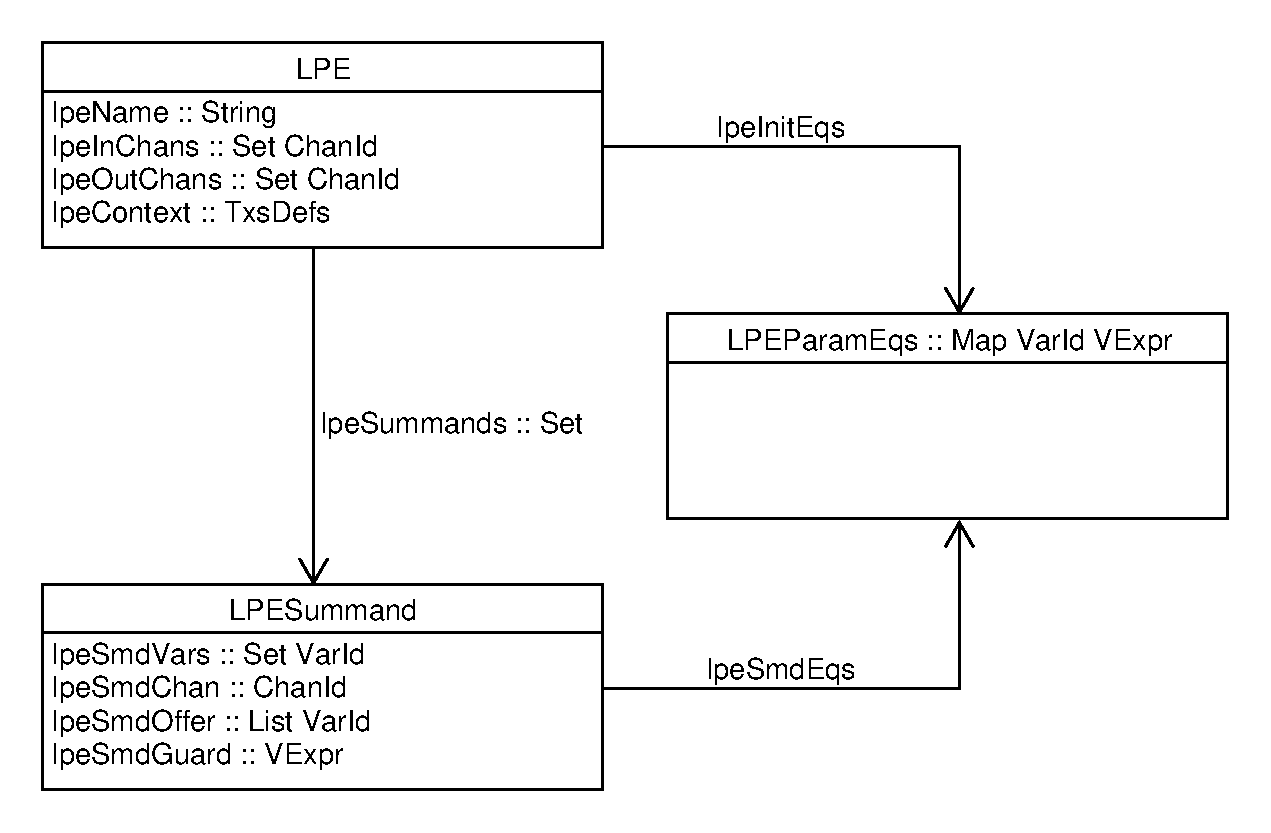
\includegraphics[width=0.7\linewidth]{images/lpe-types}
\caption{LPE data structure.}
\label{lpedatastructure:fig}
\end{center}
\end{figure}

The main data type is \texttt{LPE}, which is not a completely accurate name since it contains more information than only the linearized \txs{} process $P$, namely

\begin{itemize}
\item \texttt{lpeContext}, which is a library of \txs{} type and function definitions;
\item \texttt{lpeInChans}, which contains all channel parameters of $P$ that are input channels;
\item \texttt{lpeOutChans}, which contains all channel parameters of $P$ that are output channels; and
\item \texttt{lpeInitEqs}, which maps the data parameters of $P$ to their initial values.
\end{itemize}

The tree structure of summands that was allowed by the grammar of LPEs (see \ref{processlpeform}) has been flattened in the new data structure, resulting in a set of \texttt{LPESummand} objects that is part of the \texttt{LPE} data type.
These objects correspond with the \textit{ActionSummand} rule in the grammar.

One of the parts of the \texttt{LPESummand} data type is \texttt{lpeSmdVars}, which contains all variables that the summand uses besides LPE parameters.
These variables can be used in the channel offer, \texttt{lpeSmdOffer}, as communication variables (in a specific order); in the guard of the summand, \texttt{lpeSmdGuard}, an expression of sort \texttt{Bool}; and in the expressions that define the value of LPE parameters after the application of the summand, which are values in the \texttt{lpeSmdEqs} map.

\section{Summand elements} \label{summandelements}

To formally reference the elements of $s_i$ -- the $i$th summand of LPE $P$ -- the following definition is used:
\begin{align*}
s_i = C_i \; \texttt{?} \; x_i(1) \; \cdots{} \; \texttt{?} \; x_i(m_i) \; [[g_i]] \text{ \texttt{>->} } P(v_i(p_1), \cdots{}, v_i(p_k))
\end{align*}

where

\begin{itemize}
\item $C_i$ is the name of the channel over which summand $s_i$ communicates (if there is no such channel, \istep{} or \cistep{} is used);
\item $m_i \geq 0$ is the number of variables that summand $s_i$ uses locally, such as communication variables and hidden variables;
\item $x_i(j)$ is the $j$th variable that summand $s_i$ uses locally (communication variables first, followed by hidden variables);
\item $g_i$ is the guard of summand $s_i$ (the only free variables in this expression must be parameters of $P$, communication variables of summand $s_i$, or hidden variables of summand $s_i$);
\item $p_1, \cdots{}, p_k$ are the parameters of $P$, of which there are $k \geq 0$;
\item $v_i(p)$ is an expression that defines the new value of parameter $p$ of $P$ after the application of summand $s_i$ (the only free variables in this expression must be LPE parameters, communication variables of summand $s_i$, or hidden variables of summand $s_i$).
\end{itemize}

